% ==================================================
%
%   模型的建立与求解
%
% --------------------------------------------------

\section{模型的建立与求解}

\begin{figure}[h]
    \centering
    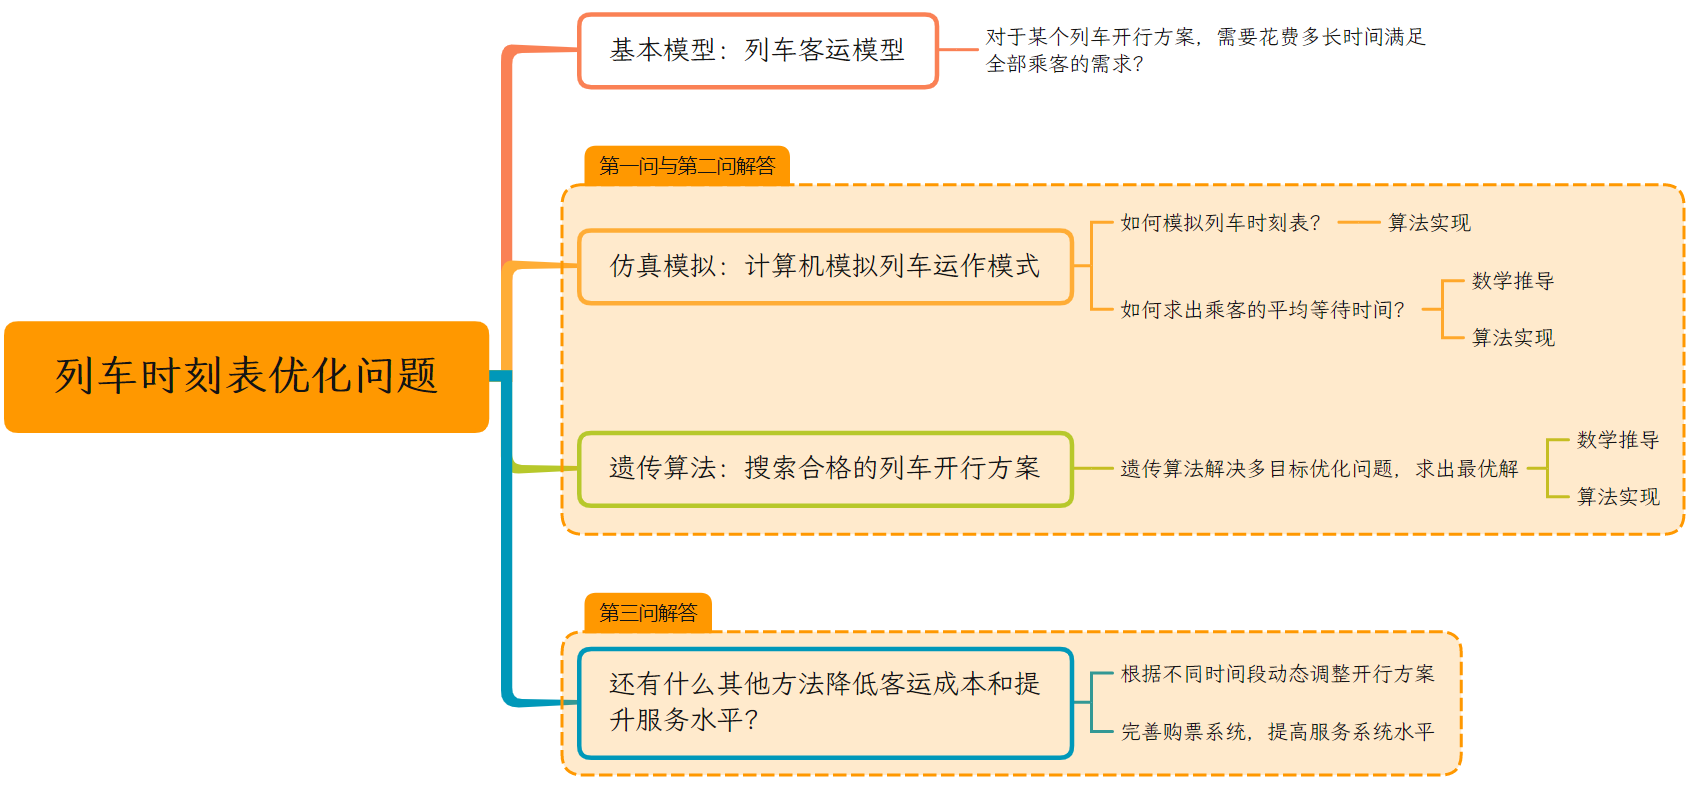
\includegraphics[scale=0.2]{res/figure161100.png}
    \caption{模型思维图}
\end{figure}

% ............ 模型的准备 ............ %

\subsection{模型的准备}

为了方便后续对问题的分析和对模型的建立,这里先给出\textbf{列车客运模型}与\textbf{遗传算法}的概述,旨在方便读者更好地理解解题模型的核心思想。

\subsubsection{列车客运模型}

列车客运模型是一种简化的列车运行模型。

为了方便表述,考虑只有$5$个车站的情况。在这$5$个车站中,从前到后依次标号为$1-5$。设发车的间隔时间为$\Delta t$,那么在该开行方案下,需要耗费多长时间才能满足所有乘客的需求?

利用列车行程图,可以清晰地展现出列车的运行模式。

\begin{figure}[h]
    \centering
    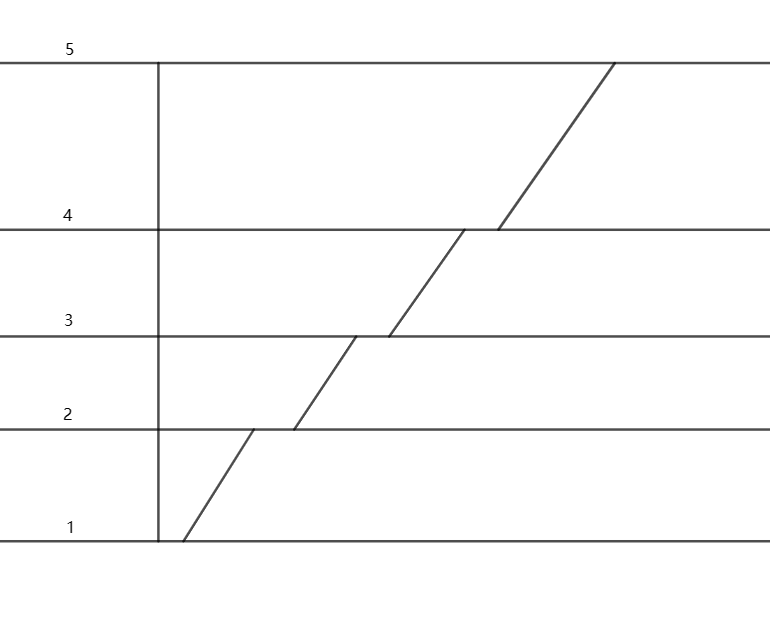
\includegraphics[scale=0.3]{res/figure160314.png}
    \caption{列车运行图}
\end{figure}

考虑现实情况以及OD客流数据,每趟列车上车的乘客是按照乘客需求的比例分配的。例如,在车站$1$时,某一次的上车乘客比例与OD客流数据比例相等。但是随着之后的列车的运行,下车的乘客数量是不一定的,即下车的时间是不一定的。为了考虑这样的情况,必须要给出很多合理的解释。这是因为原本在这个车站下车的人数就有所变化。对于这种非数值计算类问题,文后将尝试采用程序模拟的办法得到最后的运行结果,从而求出我们最开始给出的问题——需要耗费多长时间才能满足所有乘客的需求?

该模型主要功能是描述列车的运行模式,为接下来的仿真模型做好准备。

\subsubsection{遗传算法简介}

遗传算法(Genetic Algorithm, GA)也被称为进化算法(Evolutionary Algorithm)。该算法是一种仿生算法,旨在通过模仿生物遗传演化机制,达到优化群落的目的\cite{hanJiyuyichuanheshengsuanfaqiujiehanshuyouhuawenti2010}。为了更好地理解遗传算法,首先需要回顾一下自然界中生物的演化是如何进行的。

生物学表明,生物的演化是以种群为单位的,而演化的本质是基因的变异。

还有个更重要的东西——自然选择。或者通俗的理解为:种群对环境的适应度。宏观上看的话,种群是朝着适应度高的方向进行的。

根据以上论述,可以提炼出遗传算法的三个要素:

\begin{enumerate}
    \item \textbf{种群——基因与染色体},代表着种群的基本特征,是个体独特性的关键数据。在实际应用中,需要对现实问题进行编码操作;
    \item \textbf{适应度},程序模拟自然选择的重要指标。在多目标优化模型中,可以使用目标优化函数代替;
    \item \textbf{演化}。程序每一次演化,都会让种群产生新的个体。在演化的过程中,不同的基因突变和基因重组的方式,会对遗传算法的最终的效果产生极大的影响。
\end{enumerate}

在遗传算法中,首先可以用随机数算法生成初始群落。紧接着使该种群中的个体相互交配繁衍,产生新的个体。在产生新的个体的过程中,要确保完成两个操作:染色体的交叉互换和基因变异。前者保证优秀的基因有可能配对在一起;后者保证了种群的基因多样性,防止种群的基因趋同,进而防止算法陷入局部最优解。产生了下一代以后,接下来计算出所有个体的适应度,剔除适应度最低的一些个体,从而产生个体数量与初始群落一致的第二代群落。最后一次遗传算法的迭代就已经完成(如图\ref{GeneticAlgorithmDiagram})。

遗传算法迭代终止后,得到的种群就是最优解集,可以取适应度最高的解作为最终的答案。

\begin{figure}[h]
    \centering
    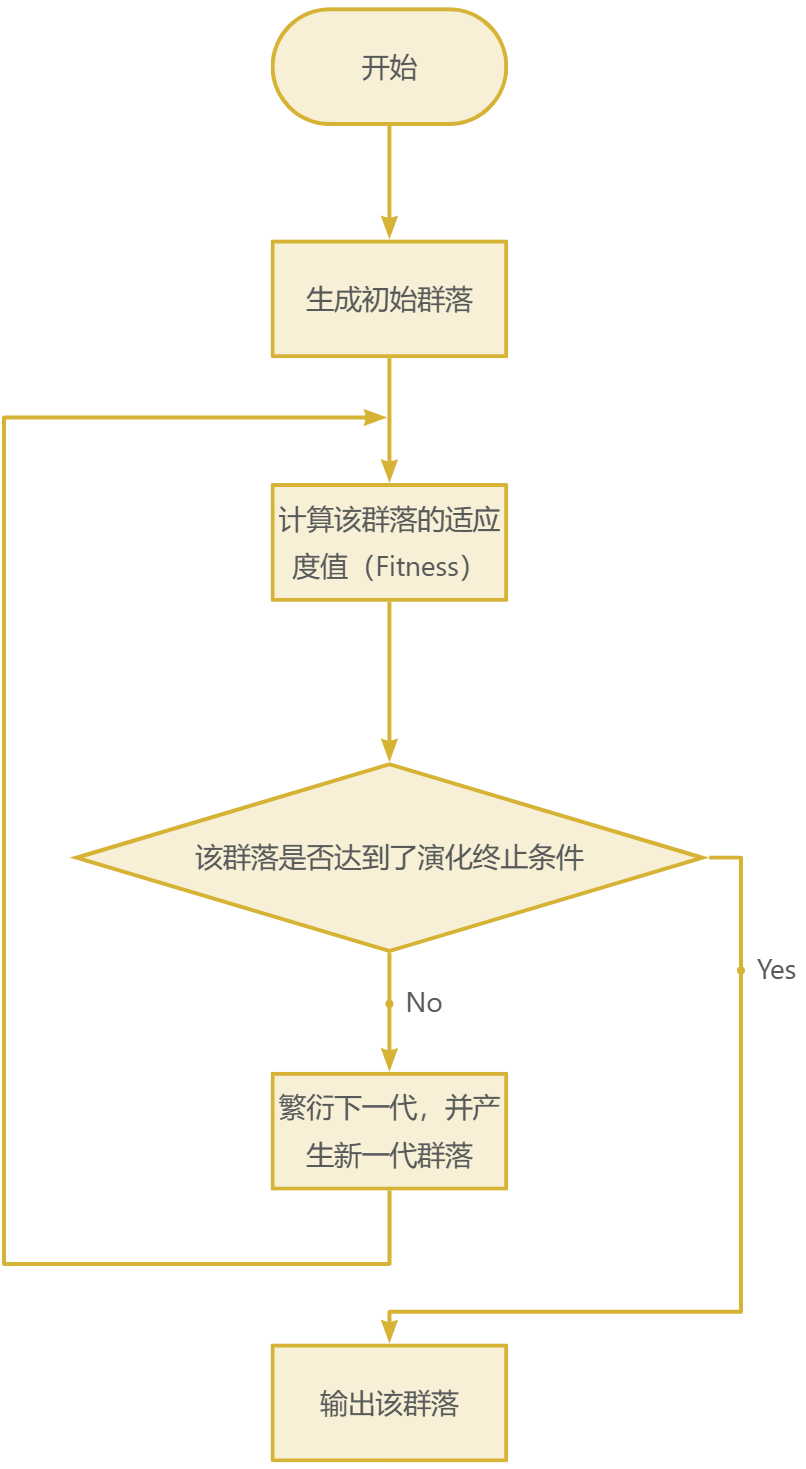
\includegraphics[scale=0.15]{res/GeneticAlgorithmDiagram.png}
    \caption{遗传算法框图}
    \label{GeneticAlgorithmDiagram}
\end{figure}

实际上,遗传算法最大的难点在于演化这一步骤。通常情况下,演化有两个重要操作需要进行——基因互换和染色体的变异。可以说,整个遗传算法的绝大部分都是对这两个操作的设计。


% ............ 模型的准备 ............ %

\subsection{问题一:仿真模拟计算与遗传算法搜索}

\subsubsection{仿真模拟计算:计算机模拟列车的运作模式}

为了确定可行的行车方案和其对应的乘客等待时间(模拟结束时间)以及企业运营成本(列车开行数量),本文考虑使用计算机枚举各种行车方案,并将对应的行车方案仿真模拟出来,判定行车方案是否可行。若方案可行,则得出其运营成本和服务水平。

本文用Python语言编写模拟代码。本模拟代码定义了三个类:Train、\newline
Station和Simulator。这三个类属性如下:

\begin{enumerate}
    \item Train
    \begin{itemize}
        \item 列车种类。
        \item 列车上的乘客总数
        \item 列车上分别到各个站点的乘客数量
        \item 列车到点时间集合
        \item 列车出发时间集合
        \item 列车运输了的乘客的总量
    \end{itemize}

    \item Station
    \begin{itemize}
        \item 车站编号
        \item 车站总上车人数
        \item 乘客目的地分布
        \item 车站未上车人数
        \item 该车站到下一车站要花的时间
        \item 该车站到下一站的距离
    \end{itemize}
\end{enumerate}

另外,Simulator类是一个模拟器。它包含了发车间隔时间、大小交路列车开行比、列车定员与安全时间间隔等参数和常量,以及当前时间、大交路列车开行数和最后发车时间等变量。此外,该类还定义了一些方法来初始化车站、规划列车和模拟运行。

在定义好几个相关的类之后,便可以开始模拟了。简单来说,模拟器通过列车客运模型模拟整个列车的运行。首先,给定最基本的参数,根据相关数据初始化模拟程序。然后进入到一层循环之中,判断站台是否还有乘客。该条件是跳出循环的关键。紧接着,又经过多次的判定和循环,最后完成模拟。具体如算法框图\ref{figure170144}所示。

\begin{figure}
    \centering
    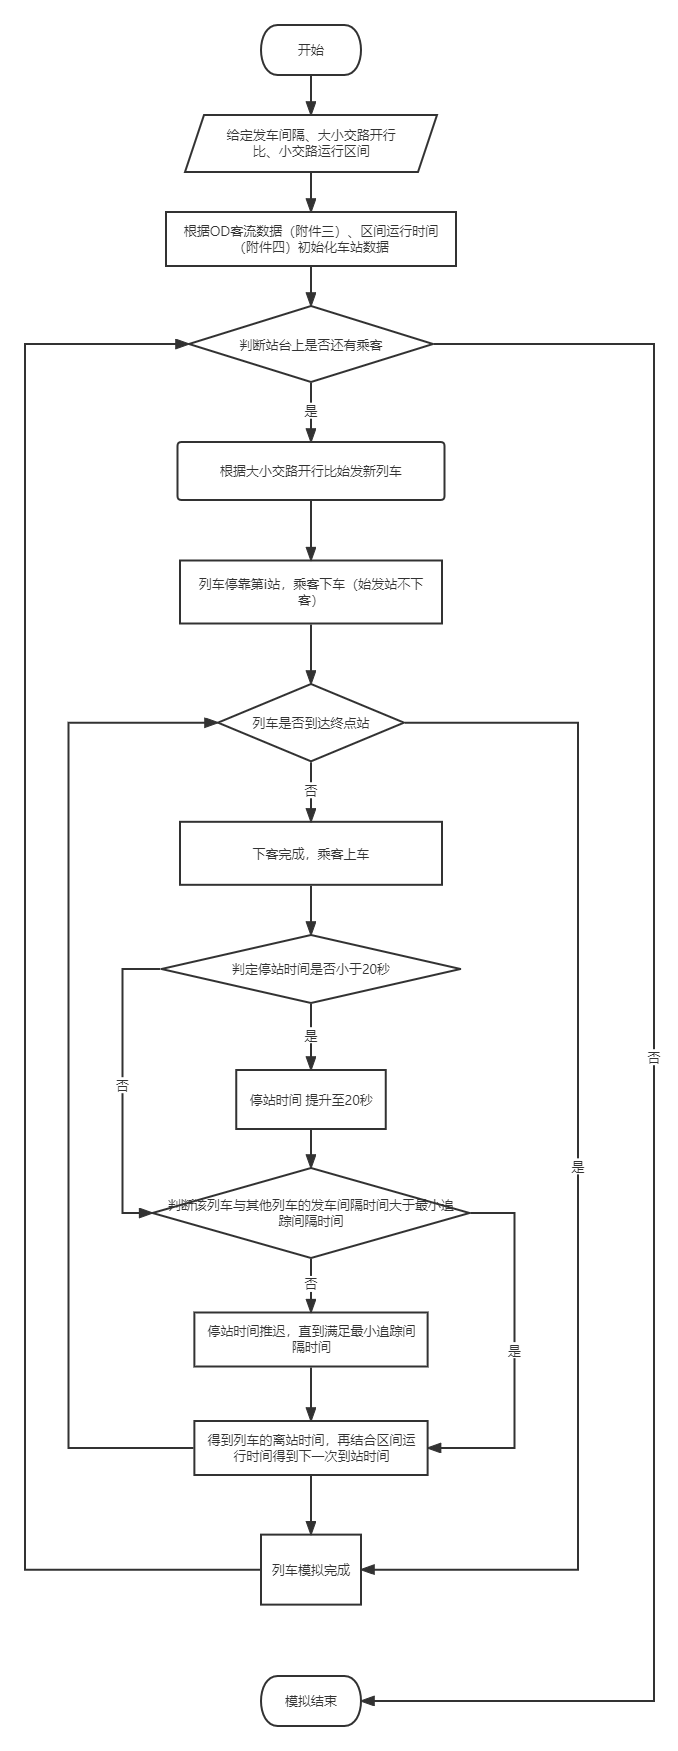
\includegraphics[scale=0.38]{res/figure170144.png}
    \caption{模拟算法框图}
    \label{figure170144}
\end{figure}

\subsubsection{求出乘客的平均等待时间}

在站台$i$,乘客去$j$站台的频率为:希望从$i$站台到$j$站台的乘客人数,与该站台总乘客人数之比。

\begin{equation}
\alpha(i, j) = 
	\frac {M_f(i, j)}{\sum _{k = i} ^{30} M_f(i, k)}
\end{equation}

第$t$辆出发的列车“刚刚”到达$i$站时,车厢内正有$M_{cur}(i, j, t)$个乘客打算到$j$站。当该车站为起点站时,列车视为“刚到”起点站,也就是乘客还未上下车。因此其初始人数为$0$,并且无论是大交还是小交均如此(大交站台$1$为起点,小交站台$s$为起点);当该车站不是起点时,刚到该车站时车厢内的乘客可以通过以下三个方面计算出来:刚到上一个站台时的车厢状态、上一个站台的下车乘客和上一个站台的上车乘客。

\begin{equation}
M_{cur}(i, j, t) = 
	\begin{cases}
	M_{cur}(i - 1, j, k) - M_{out}(i - 1, t) + M_{in}(i - 1, j, t)  & \text{ if }\sigma \\
	0  & \text{ ow }
	\end{cases}
\end{equation}

其$\sigma$为条件区域:

\begin{equation}
    \sigma = 
        \begin{matrix}
 		1 < i \leq 30, (t - 1) < N_l \mod (N_l + N_s),  \\
		\text{ or } s < i \leq e, (t - 1) \geq N_l \mod (N_l + N_s)\\
		\end{matrix} \\
\end{equation}

当第$t$辆发车的列车到第$i$个站台时,无论乘客的起点在哪,在该站台下车的乘客都会下车,即下车人数为:列车刚到这一站台时,所有目标在这一站台下车的本列车乘客总数,并且无论乘客是乘坐大交还是乘坐小交都是这样。特别地,由于小交的范围不会超过大交的范围,因此:当小交到达不在运行范围内的车站时,其下车乘客人数视为$0$。

\begin{equation}
M_{out}(i, t) = 
	\begin{cases}
	\sum _{k = 1} ^{i} M_{cur}(k, i, t)  & \text{ if } (t - 1) < N_l \mod (N_l + N_s) \\
	\sum _{k = s} ^{i} M_{cur}(k, i, t)  & \text{ if } s \leq i \leq e, (t - 1) \geq N_l \mod (N_l + N_s) \\
	0 & \text{ otherwise }
	\end{cases}
\end{equation}

提示:由于假定滚动发车从大交开始,第一个发车的列车无论何时一定是大交而绝对不会是小交。

对于任何一辆列车来说,主要有三个条件限制了乘客上车人数:一是列车本身的容量,即列车中乘客总数不能超过列车定员数。为了计算这一点,首先要计算出:该列车到达这一站,乘客下车后还剩多少个乘客还在车上。经过计算,车上的乘客数量最多不能超过:刚到该站的列车乘客状态与所有下车的乘客数之差,即:

\begin{equation}
C = \sum _{k = i} ^{30} M_{cur}(i, k, t) - M_{out}(i, t)
\end{equation}

那么就可以算出最多还可以容纳的乘客数量为:

\begin{equation}
    V_{max_1} = V-C
\end{equation}

其中$V$为定员数。

除了容量限制外,还有时间限制乘客上车人数,即当超过一定时间后列车门将关闭,并且不再允许上车。除去下车用时,最多还能上车的乘客数量为:

\begin{equation}
V_{max_2} = \frac {t_{max}} {t_{avg}} - M_{out}(i, t)
\end{equation}

与此同时,该站台的人数也会影响上车人数,即当该站台人数不能填满列车时,列车还应该有多余空位,而该车站却已无其他乘客(已经被其他的列车接走了)。因此,最多上车乘客数量为:

\begin{equation}
V_{max_3} = \sum _{k = i} ^{30} M_f(i, k) - \sum _{k = 1} ^{t - 1} \sum _{l = i} ^{e} M_{in}(i, l, k)
\end{equation}

总之,我们对以上结果取最小值,即第$t$列开行的列车在站台$i$的实际上车总人数为$\max _{i = 1} ^{3} \{V_{max_i}\}$。

接下来还需要考虑上车的乘客分别要去往哪个站台。而乘客上下车不会影响该站台不同目的地的乘客比例,因此对总人数乘以对应的数量频率即可得到答案。

以上算的都是针对大交的,至于小交,只需修改求和范围即可(当然,对于小交不运行的范围,对应上车乘客数视为$0$)。

\begin{equation}
M_{in}(i, j, t) = 
	\begin{cases}
	\min \left\{
	 	V - F(30), \quad
	  	Q, \quad
	  	\sum _{k = i} ^{30} M_f(i, k)
	\right\} \cdot \alpha(i, j) &  FI_1\\
	\min \left\{
	 	V - F(30), \quad
	  	Q, \quad
        G(30)
	\right\} \cdot \alpha(i, j) &  FI_2\\
	\min \left\{
	 	V - F(e), \quad
	  	Q, \quad
        G(e)
	\right\} \cdot \alpha(i, j) &  FI_3\\
	0 & \text{ ow } 
	\end{cases}
\end{equation}

其中,$FI_i(i=1,2,3)$分别代表:

\begin{equation*}
    \begin{cases}
        FI_1 = \text{if}(t-1)<N_l\mod(N_l+N_s), t = 1  \\
        FI_2 = \text{ if } (t - 1) < N_l \mod (N_l + N_s), t > 1    \\
        FI_3 = \text{ if } (t - 1) \geq N_l \mod (N_l + N_s), s \leq i, j \leq e \\
    \end{cases}
\end{equation*}

$F(x)$、$G(x)$、$Q$代表:

\begin{equation*}
    \begin{cases}
        F(x) = \sum _{k = i} ^{x} M_{cur}(i, k, t) - M_{out}(i, t)  \\
        G(x) = \sum _{k = i} ^{30} M_f(i, k) - \sum _{k = 1} ^{t - 1} \sum _{l = i} ^{30} M_{in}(i, l, k)   \\
        Q = \frac {t_{max}} {t_{avg}} - M_{out}(i, t)   \\
    \end{cases}
\end{equation*}


第一个开行的车一定不是小交,因此暂时不用考虑追踪时间。而由定义得,第一个车从起点开始行驶发生在乘客上下车完成后。而由于实际的上下车的数据均已知,因此可以利用平均一人上下车时间得到该车出发的时间。而对于下一个站的出发时间,只要用当前站的时刻,加上到下一站的耗时,再加上下一站的乘客上下车时间即可。

由于采取“先规划后行驶”的方案,规划完第一个车的时刻后再考虑下一辆车。

对于下一辆车,要么是小交、要么是大交,可能会受到追踪时间干扰。但是前提是在同一区间,即假设发车前有车还没有到达下一个站台,因此必须考虑那辆车是“什么时间”出发的,即选择“同一车站中,发车时间最近的那一辆列车”判断是否超过追踪时间。当超过追踪时间后才可以发车。因此,本列车的出发时刻为:乘客上下完车后的时刻、最近的那辆车从本站出发的时刻再加上追踪时间,取最大值。

\begin{equation}
M_{tm}(i, t) = 
	\begin{cases}
		t_{avg} \cdot \sum _{k = i} ^{30} M_{in}(i, k, t) &  FI_1\\
		H & FI_2\\
		\max \left\{ 
			H, \quad
			\max _{k = 1} ^{t - 1}M_{tm}(i, k) + t_{del}
		\right\} & FI_3\\
		 \\
		0 & \text{ ow }
	\end{cases}
\end{equation}

其中,$FI_i(i=1,2,3)$分别代表:

\begin{equation*}
    \begin{cases}
        FI_1 = \text{ if } i = t = 1   \\
        FI_2 = \text{ if } i > 1, t = 1    \\
        FI_3 = \text{ if }\begin{matrix}
            t > 1, (t - 1) < N_l \mod (N_l + N_s),  \\
            \text{ or } s \leq i \leq e, t > 1, (t - 1) \geq N_l \mod (N_l + N_s)
            \end{matrix}
    \end{cases}
\end{equation*}

$H$代表:

\begin{equation*}
    H = M_{tm}(i - 1, t) + t_{i - 1} + t_{avg} \cdot \left[
			M_{out}(i, t) + \sum _{k = i} ^{30} M_{in}(i, k, t)
		\right]
\end{equation*}

由于$M_{tm}$的意义为列车刚离开的时间,也就是列车乘客刚上下车结束后的时间,因此最长的那个是最后一个完成任务的,于是最后完成的时间即为答案。

\begin{equation}
t_{total} = \max _{i, t} \{M_{tm}(i, t)\}
\end{equation}


\subsubsection{遗传算法解双目标规划模型}

\paragraph{双目标规划模型}

企业运营的成本可以分为两类,分别运营固定成本与变动成本。其中运营的固定成本为列车的采购数量,而变动成本为列车的运行总里程。于是,可以建立双目标规划模型\cite{caoJiyuchengkedengdaishijiandechengshiguidaojiaotongliecheshikebiaoyouhuamoxingyusuanfayanjiu2021}:

\begin{equation}
    \min Z = \min z_1 + \min z_2
\end{equation}

根据最短理想点法,存在评价函数:

\begin{align}
    U = (z_1, \cdots, z_m) = \sqrt{\sum_{j=1}^m(z_j-z_j^{\min})^2}  \\
    U^{'} = (z_1, \cdots, z_m) = \sqrt{
        \sum_{j=1}^m (
                \frac{z_j-z_j^{\min}}{z_j^{\min}}
            )^2
        }
\end{align}

故有:

\begin{equation}
    Z = U^{'}=(z_1,\cdots,z_m)
\end{equation}

\paragraph{遗传算法流程}

根据前文的分析,下面依次给出再该问题中,遗传算法的三要素的具体值:

\begin{enumerate}
    \item \textbf{种群}。大小交路车次之比$x$,小交路起始点与终点向量$(a_i, a_j)$,发车频率$f$。所以种群的编码为两个数字和一个向量。
    \item \textbf{适应度}。在本文中,定义$f(x)=Z(x)$。
    \item \textbf{演化}。在演化过程中,主要有下面几个关键点:
    \begin{itemize}
        \item 采用择优保存法。把每一代中适应度最高的个体原封不动的保存下来,这样可以防止基因的不确定性,导致整个种群的适应度降低;
        \item 只有对应的数据基因可以进行染色体的交叉互换;
        \begin{figure}[h]
            \centering
            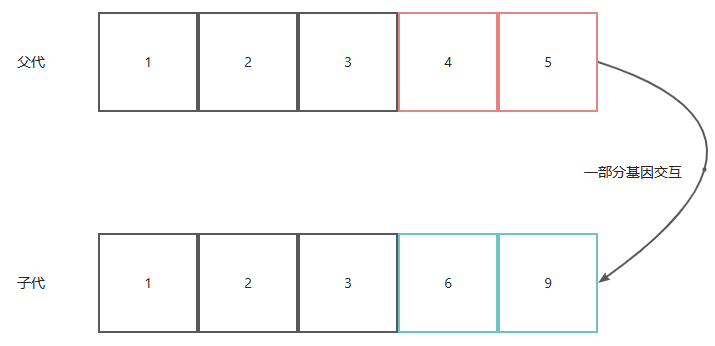
\includegraphics[scale=0.4]{res/figure170220.png}
            \caption{染色剂交叉互换}
            \label{figure170220}
        \end{figure}
        \item 对于基因突变,本文的遗传算法中采用单点突变法。对于给定的变异概率$p$,然后根据对于的变异函数,突变为一个新的值(如图\ref{figure170202})。
        \begin{figure}[h]
            \centering
            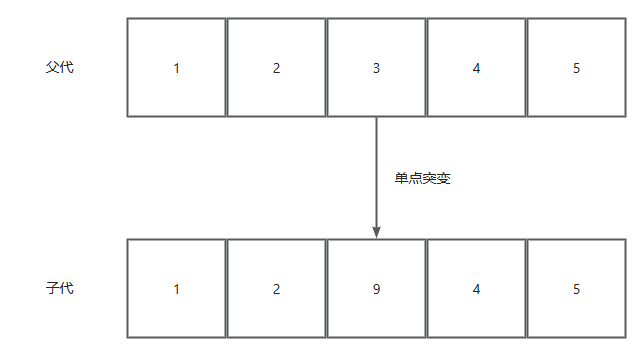
\includegraphics[scale=0.4]{res/figure170202.png}
            \caption{单点突变}
            \label{figure170202}
        \end{figure}
    \end{itemize}
\end{enumerate}


\paragraph{计算结果}

经过前文的分析和定义以后,便可以导入数据计算了。在这里将分别导入OD客流数据以及区间运行时间这两份数据。最后求得结果如下表。

\begin{table}[h]
    \centering
    \caption{计算结果}
    \begin{tabular}{cccc}
    \hline
        & 运行区间     & 运营里程   & 开行数量 \\ \hline
    大交路 & $1$号站-$30$号站 & $80.216$ & $2$    \\
    小交路 & $8$号站-$25$号站 & $480.936$ & $24$   \\ \hline
    \end{tabular}
\end{table}

% ............ 模型的准备 ............ %

\subsection{问题二:等间隔的平行运行图}

通过前文中的仿真模拟算法,可以得出相对应的平行运行图。绘制等平行运行图的原则是“前车优先”。从前往后,依次绘制车的运行模式。

首先,设置一个车次计数器。没发出一辆车就增加一个。当规划第一趟车的时候,可以没有顾虑地规划。接下来依次发车,接下里发出地每趟车,都要经过冲突检验,即判断当前车次是否会与以后的车次发生冲突,如无冲突,则规划下一趟车,否则适当推出改的时刻表。

经过上面的算法循环以后,可以得到相对应的列车等间隔平行运行图。算法如图\ref{figure170309}所示。

\begin{figure}[h]
    \centering
    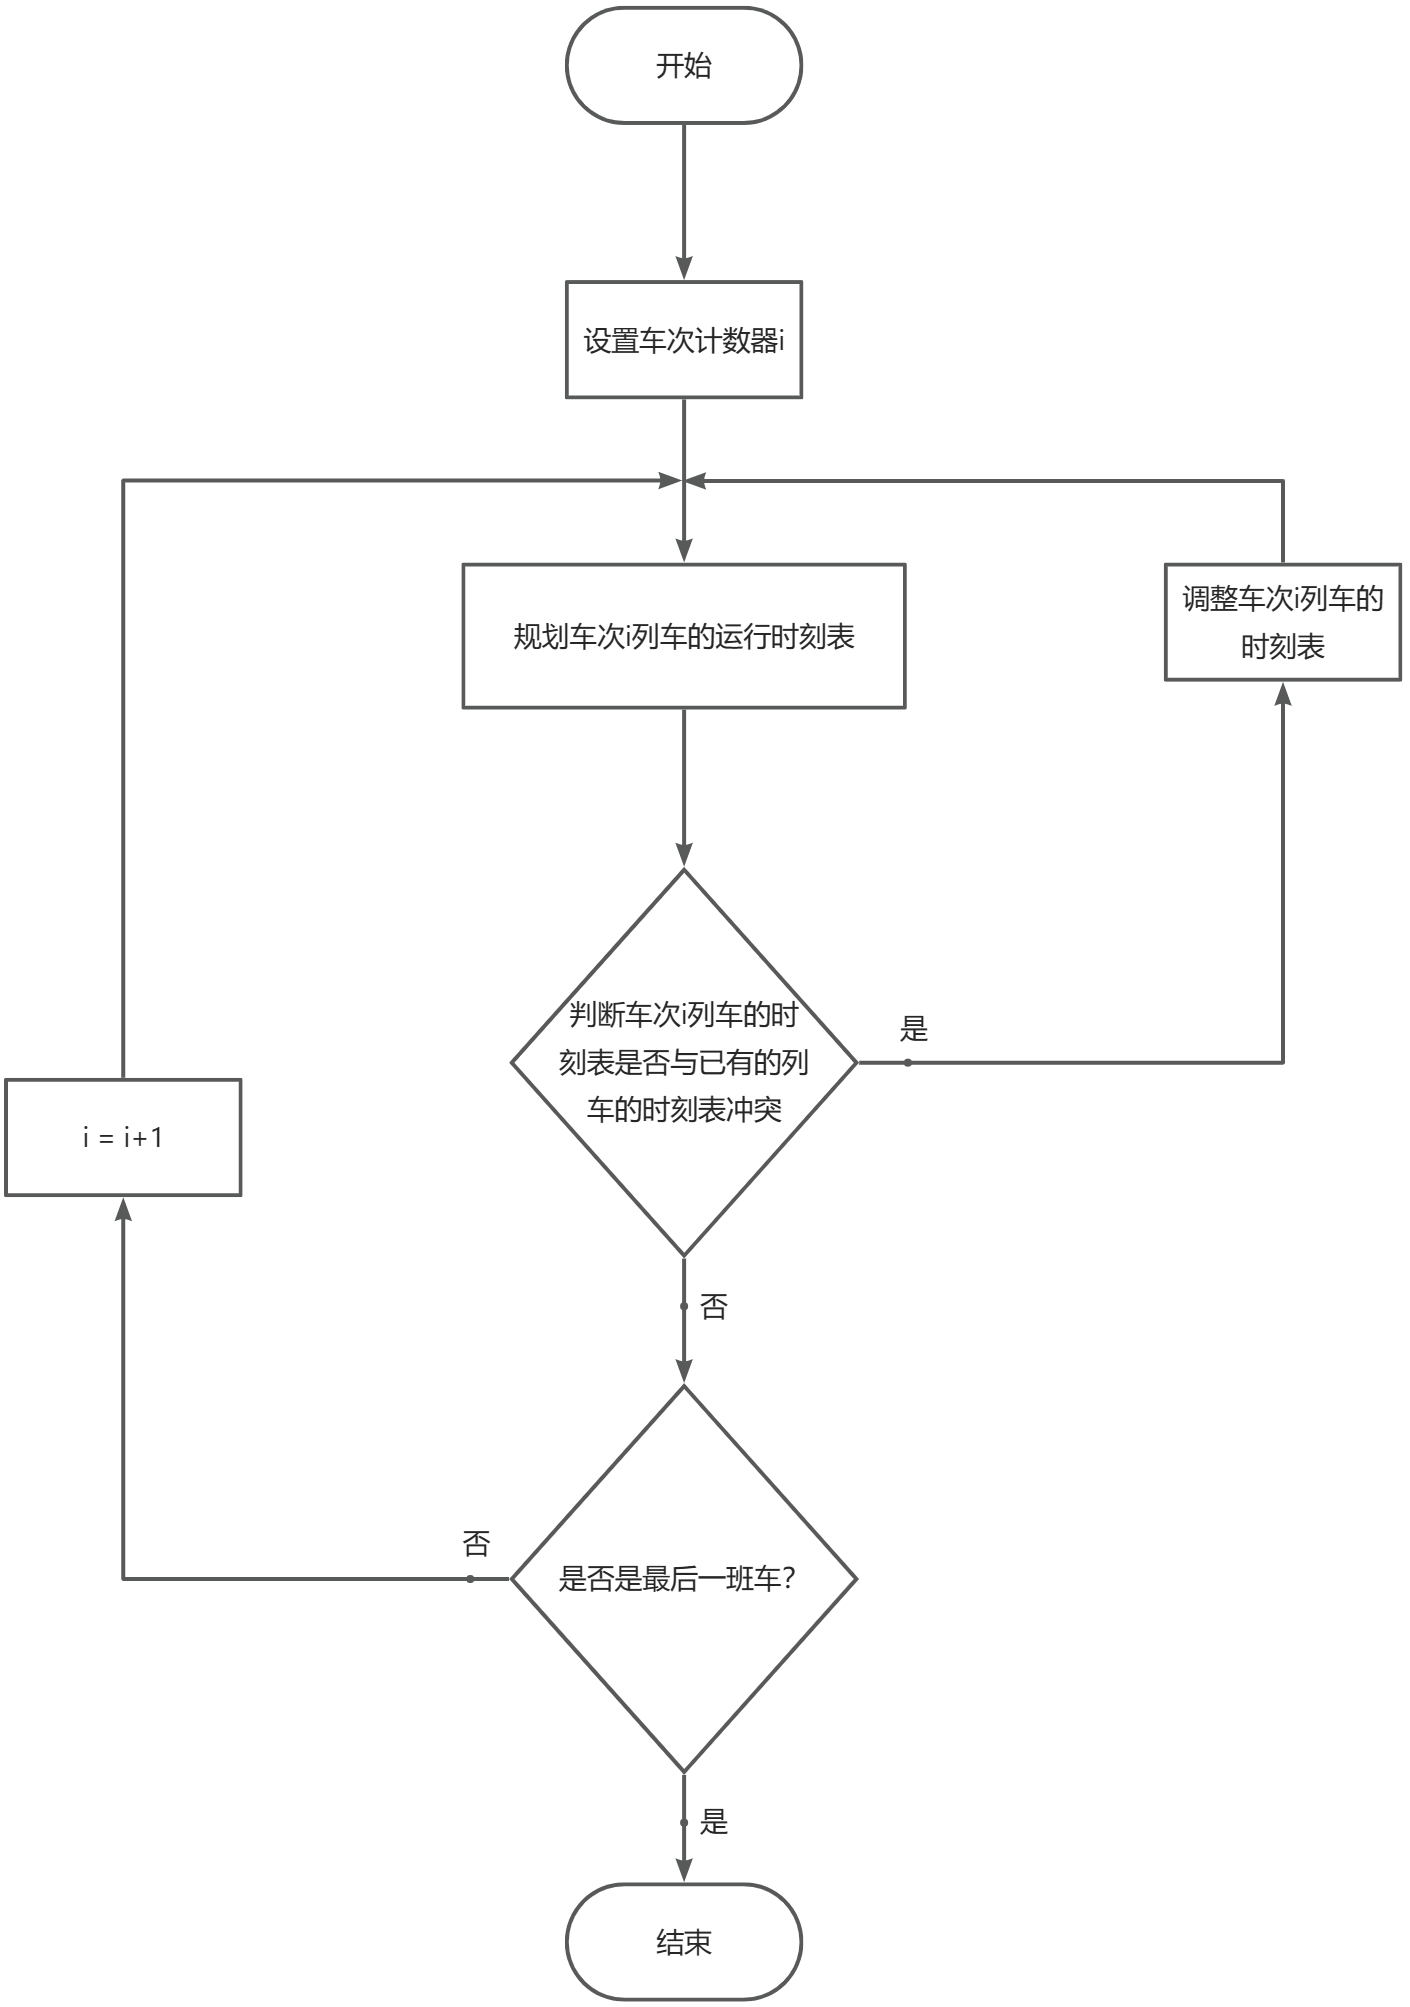
\includegraphics[scale=0.2]{res/figure170309.png}
    \caption{平行运行图算法}
    \label{figure170309}
\end{figure}

\subsection{问题三:针对不同时间段动态调整列车开行方案}

\subsubsection{列车开行方案调整的背景}

从中华人民共和国交通运输部公布的数据中可以看出来:2023的1-2月份的旅客数量明显增加\cite{ChengShiKeYunTongJiShuJuZhongHuaRenMinGongHeGuoJiaoTongYunShuBu}。其原因一方面是日近春节,人们需要回家;另一方面是疫情放开,在家中憋了很多时间的人也逐渐开始旅游,回归正常生活。

正因如此,随着疫情控制逐渐放开,列车的运营方案选择显得越来越重要。企业如果不能及时更新列车运营方案而用疫情时期的旧运营方案,很有可能造成其运营成本增加和列车服务质量降低等各种问题,从而间接减少企业利润。因此,对于一个企业来说,应当及时调整列车运营方案以增加利润。

\subsubsection{列车开行方案调整思路}

对于如何调整列车运营方案,应当针对不同时间段动态调整列车开行方案。接下来对不同情况时的客流量进行分析,方便提出相应的列车开行方案调整思路:

对于不同的日子,乘客们对列车的交通需求是不一样的。例如:在工作日中,需要用列车作为交通工具的人数较少;而在节假日中,列车作为一个重要的交通工具,可以让乘客去往各个不同的地方旅游或让乘客从各个地方回到家中。

与此同时,对于不同的站点,其客流量也不同。比如说:在节假日,由于某一站点可以更方便地到达一些著名景点或者“网红打卡胜地”,许多人在旅游时都会从其他各个站台涌入该站台;从节假日回到工作日时,许多乘客们都会从该站台返回到其他各个站台继续工作。

为了应对不同站点不同时间客流量时多时少的情况,应当动态地调整列车开行方案,减少企业运营成本,提高列车服务质量。

\subsubsection{工作日的列车开行方案调整}

在工作日中,大部分人都在工作,因此需要乘车的人数不多。在列车开行方案中,应当优先考虑运营成本,其次考虑列车服务质量,即在考虑列车开行方案时,应优先考虑运营成本,其次考虑列车服务质量。

由于工作日时客流量不大,用大交路的运营模式即可。如果采用大小交路的运营方式,可能造成多辆“空车”运营,增加不必要的企业运营成本。

总之,对于工作日,应当采用大交路的运营方式,着重考虑企业的运营成本。

\subsubsection{日常节假日的列车开行方案调整}

在日常节假日,许多乘客因不同原因有乘坐列车的需求,其中以出门旅游为原因的乘客居多。而在列车开行方案中,应当优先考虑列车服务质量,其次考虑运营成本,即列车服务质量的权重应大于企业运营成本的权重。

在列车实际运营时,前往著名景点附近车站的乘客,其人数往往会特别多,即很多乘客会从其他各个站台集中到某个站台;不仅如此,还有可能出现乘客们集中去往多个其他站台的情况。当然,在节假日结束时,还会出现乘客从集中的一个或几个站台分散到其他站台。对于这些乘客集中进站的特殊情况,需要专门制定列车开行方案。

如果只使用大交路运营,制定方案极其有限,很难从中找出合适的方案应对这种情况。因此,应当考虑大小交路的运营模式。

由于大交路的运营范围是确定的,小交路的运营范围应该尽可能缩小,并且把旅游景点站台包括进去,加快与景点站台相邻的站台的乘客流动,防止出现在某一站台出现乘客过多的情况。

总之,对于日常节假日,应当采用大小交路的运营方式,使小交路的运营范围应尽可能小,并且把著名景点所在的车站尽可能覆盖。

\subsubsection{春节假期的列车开行方案调整}

在春节这一特殊的节假日,乘客去往各个站台的人数较为平均。虽然实际上其与对应地区的人数有关,但是乘客数量依旧十分庞大,这恰与工作日截然相反。

因此应当采用大小交路的运营模式。由于大交路的运营范围是一定的,为了分摊大交路的乘客运送,小交路的范围在这种特殊情况下应当适当增加。当然小交路的范围不能与大交路一样,否则不能体现大小交路的优势。于是考虑小交路的起终点应当与大交路的起终点较为接近较为合适。这种列车开行方案不仅能让小交路为大交路分摊客流量,还可以为乘客考虑换乘路线、给乘客提供更多的选择。

总之,对于春节假期,应当采用大小交路的运营方式,并且小交路的起终点因与大交路的起终点较为接近。


% ==================================================
%
%   模型的评价与改进
%
% --------------------------------------------------

\section{模型的评价与改进}

\subsection{模型的优点}

\begin{enumerate}
    \item 该模型充分考虑乘客在现实中的情况,各种类型的乘客随机上车,每个车站的乘客类型分布都不同;
    \item 该模型考虑了各个列车行驶的路径,并且能够自动调整列车的冲突,确保列车安全运行;
    \item 该模型通过优化算法极大的降低了时间复杂度,提高了求解答案所需要的时间。
\end{enumerate}

\subsection{模型的缺点}

\begin{enumerate}
    \item 该模型只考虑了某个时间上的状态,对于其他时候的安排需要另行设计;
    \item 该模型只能求得近似最优解,甚至在某些情况下,只能求出局部最优近似解,而没有全局最优解;
    \item 该模型难以适应突发状况,一旦有列车的晚点,整个结论就必须要重新计算。
\end{enumerate}

\subsection{模型的推广}

\begin{enumerate}
    \item 该模型中应用了遗传算法。遗传算法可以用来解决NP类问题,利用概率从一个超大集合中搜寻到某个满足条件的解。该算法应用场景广泛,譬如再商旅路径问题中也有应用;
    \item 该模型中使用提出了一种列车客运模型,可以用来描述列车的运动状态,使用该模型,可以充分考虑各个列车之间的间隔对列车行驶带来的影响。
    \item 该模型中设计了一套算法用来模拟列车的运行状态,以求出列车的时刻表。计算机的模拟可以用来解决很多复杂的现实,再一定情况下,适当使用计算机模拟是一种很好的方法。
\end{enumerate}